% Created 2024-08-04 Sun 16:33
% Intended LaTeX compiler: pdflatex
\documentclass[letterpaper,tgtermes,9pt,microtype,colorlinks=true,urlcolor=blue,DIV=calc,pagesize]{scrartcl}
\usepackage[utf8]{inputenc}
\usepackage[T1]{fontenc}
\usepackage{graphicx}
\usepackage{longtable}
\usepackage{wrapfig}
\usepackage{rotating}
\usepackage[normalem]{ulem}
\usepackage{amsmath}
\usepackage{amssymb}
\usepackage{capt-of}
\usepackage{hyperref}
\KOMAoptions{parskip=half-,headings=small}\usepackage[normalem]{ulem}
\usepackage[usenames,dvipsnames,svgnames,table]{xcolor}
\areaset{6.5in}{9.2in}%\usepackage[margin=1in]{geometry}
\usepackage{fancyhdr}
\usepackage{enumitem}\setlist{itemindent=1ex,listparindent=1ex}
\setlist{noitemsep,topsep=0pt,parsep=0pt,partopsep=0pt}
\setlist[enumerate,1]{label=\alph*.,ref=\alph*}
\setlist[enumerate,2]{label=\arabic*),ref=\theenumi.\arabic*}
\setlist[enumerate,3]{label=\alph*),ref=\theenumii.\alph*}
\setlist[enumerate,4]{label=(\arabic*),ref=\theenumiii.\arabic*}
\newcommand{\classmark}{UNCLASSIFIED -- FOR TRAINING ONLY}
\newcommand{\ordershorttitle}{OPORD 24-01}
\newcommand{\ordertitle}{OPERATION ORDER 24-01 OPERATION TYPESET (\classmark)}
\fancypagestyle{plain}{\fancyhf{} \fancyhead[L]{\ordershorttitle}%
\fancyhead[C]{\classmark{}}\fancyfoot[C]{\classmark{}\\\thepage}}
\author{George Allen}
\date{\today}
\title{}
\begin{document}

\textcolor{red}{This is a sample document to show how org-mode and LaTeX can generate formatted PDFs, using an Army OPORD as an example. \textbf{It does not claim to be well-structured, doctrinally correct, or even useful.} It's just an example.}

\textcolor{red}{As an additional caveat, don't expect anyone ever to collaborate with you using this workflow. Again, this is just an example of what can be done. However, Emacs org-mode provides an excellent tool for note-taking, task tracking, and many other tasks. The same technique used in this document, with the addition of appropriate bibliography and formatting packages, can generate Chicago, APA, and other formats for research papers.}

\raggedright

\pagestyle{plain}
\begin{flushright}
UNIT\ldots{}\\
LOCATION\ldots{}\\
\today\\
\ordershorttitle\\
\end{flushright}

\widowpenalty1000
\clubpenalty1000
\raggedbottom

\textbf{\ordertitle}

\emph{(Example using org-mode \texttt{->} \LaTeX{} \texttt{->} PDF to format an OPORD. ORDER based on example from GTA 07-10-003 Infantry Reference Card for Small Unit Leaders (Nov 2021).}

\textbf{Task Organization:}

\emph{Describe the allocation of forces to support the commander's concept.}

\textbf{Weather:} Weather and Light Data and General Forecast:

\begin{center}
\begin{tabular}{rrrllr}
High & Moonrise & Sunrise & Wind Speed & Moonphase & BMNT\\
89 & 0342 & 0652 & 5mpg & New & 0552\\
Low & Moonset & Sunset & Wind Direction & \% Illumination & EENT\\
73 & 1900 & 0834 & NE & 0.1 & 2134\\
\end{tabular}
\end{center}

(Discuss the effects on friendly and enemy – for example, how does it affect
your mission.) Visibility: Does it favor attacker or defender (illumination \%
and so forth)?  Wind: Speed and direction (effects on obscuration and chemical,
biological, radiological, and nuclear [CBRN]). Precipitation: Effects on
trafficability, visibility, CBRN, and obscurants.  Cloud Cover: Effects on
aviation, visibility, and laser-guided munitions. Also, certain conditions
enhance obscurant and chemical use.

Temperature: Effects on personnel and equipment use; air density affects
aviation payloads and smoke operations.

\textbf{Terrain:} Analyze using the military aspects of terrain; obstacles, avenues of
approach, key terrain, observation and fields of fire, and cover and
concealment (often expressed in the Army memory aid OAKOC). The leader
determines the effects of each aspect of terrain on both friendly and enemy
forces. These effects translate directly into conclusions that can apply to
friendly or enemy COAs. This procedure is to first identify where forces have
difficulty moving (obstacles) then identifying areas where forces can travel
(avenues of approach) become more evident. Leaders may analyze “OAKOC” in any
order they choose.

\begin{itemize}
\item \textbf{Obstacles:} Identify both existing and manmade obstacles, specifically
highlighting those on/around the objective.
\item \textbf{Avenues of approach:} Identify routes (air, ground, mounted, dismounted) of
attacking forces leading to their objectives or key terrain.
\item \textbf{Key terrain:} Identify terrain that provides a marked advantage to whomever
controls it. If present, identify DECISIVE TERRAIN that must be controlled
for success of the unit.
\item \textbf{Observation/fields of fire:} Identify areas that provide observation and
engagement possibilities for direct and indirect fire systems. Focus on
identifying such positions in and around the objective, for both friendly
and enemy forces. Locate intervisibility lines: terrain that prevents
observation from one point to another.
\item \textbf{Cover and concealment:} Identify positions that provide cover (protection
from fire) and concealment (protection from observation). Positions of cover
can often be found on the forward slope of intervisibility lines.
\end{itemize}

(Discuss the effects on friendly and enemy in your area of operations –for
example, how does it affect your mission.)
\section{\textbf{SITUATION}}
\label{sec:org1de75d2}

\begin{enumerate}
\item \textbf{Enemy Forces:}
\label{sec:org1ddd9c7}
\begin{enumerate}
\item The enemy situation in higher headquarters’ OPORD (paragraph 1.a.) is the basis for this, but the leader refines this to provide the detail required by hissubordinates. Include enemysupport from higher,which may affect your mission.
\begin{enumerate}
\item Composition: Identify the enemy we are facing using (if available) enemy order of battle diagrams. (What is the enemy's task organization?) Also, identify the enemy's equipment (weapons and ranges, night vision device and more). Describe the number of enemy (STRENGTH) and number of weapons available.
\item Disposition: Where is the enemy and his weapon systems located? What is the enemy’s mission? (Point to map or how on sand table.) Include both known and suspected locations.
\item Capabilities: What CAN the enemy do?
\item Recent Activities: Describe the enemy's most likely COA. If possible, use a sketch or sand table to aid in this description
\end{enumerate}
\end{enumerate}
\item \textbf{Friendly Forces:}
\label{sec:orged74745}
This information is in paragraph 1b, 2 and 3 of higher headquarters’ OPORD.
\begin{enumerate}
\item Include the mission, the commander's intent, and concept of operations for
headquarters one and two levels up.
\item Identify the locations of units to the left, right, front, and rear. State
those units’ task and purpose and how those units will influence your unit, particularly adjacent unit patrols.
\end{enumerate}
\item \textbf{Attachments and detachments.}
\label{sec:org1d23598}
Do not repeat information already listed under task organization. Try to put all information in the task organization. However, when not in the task organization, list units that are attached or detached to the headquarters that issues the order. State when attachment or detachment is to be effective if different from when the OPORD is effective (such as on order, on commitment of the reserve). Use the term “remains attached” when units will be or have been attached for some time.
\end{enumerate}
\section{\textbf{MISSION}}
\label{sec:orgadaca35}
The leader concludes mission analysis by restating the mission. A mission statement is a short sentence or
paragraph that describes the organization’s essential task(s), purpose, and action containing the elements of who, what, when, where, and why. The five elements of a mission statement answer these questions, commonly referred to as the five Ws: Who will execute the linkup operation (unit or organization)? What is the unit’s essential task (linkup, tactical mission task)?
\section{\textbf{EXECUTION}}
\label{sec:org49ae2f1}
\begin{enumerate}
\item \textbf{Commanders Intent}
\label{sec:orge4988c8}
The commander’s intent is a clear, concise statement of what the unit must do and conditions the unit must establish with respect to the enemy, terrain, and civil considerations that represent the desired end state.
\begin{itemize}
\item When will the operation begin (by time or event) or what is the duration of the operation?
\item Where will the operation occur (linkup point[s], area of operations, objective, grid coordinates)?
\item Why will the force conduct the linkup operation (for what purpose)?
\end{itemize}
\item \textbf{Concept of operations.}
\label{sec:orge1df4cd}
The concept of operations may be a single paragraph, may be divided into two or more subparagraphs or, if unusually lengthy, may be prepared as a separate annex. The concept of operation is based on the COA statement generated during the third step of the troop-leading procedures. The concept statement should be concise and understandable, and describe in general terms how the unit will accomplish its mission from start to finish.
The concept—
\begin{itemize}
\item Describes the employment of maneuver elements in the form of a concept statement.
\item Identifies by subunit the main effort and supporting efforts.
\item Describes a general plan of fire support or “scheme of fires” supporting movement and maneuver with fires.
\item Describes the integration of other elements or systems within the operation. These include, for example, reconnaissance forces, surveillance assets, security forces, intelligence operations, engineers, and air defense.
\end{itemize}
\item \textbf{Scheme of movement and maneuver.}
\label{sec:orgf3bab83}
This paragraph addresses, in detail, the mechanics of the operations. Specifically address all subordinate units and attachments by name, giving each its mission in the form of a task and purpose. The main effort must be designated and all other subordinates ’ missions must relate to the main effort. (At the squad level, actions on the objective will comprise the majority of this paragraph and therefore could address the plan for actions on the objective, engagement/disengagement criteria, an alternate plan in the event of compromise or unplanned movement of enemy forces, and a withdrawal plan. In other words, all actions of this unit from start of mission until completion.)
\item \textbf{Scheme of fires.}
\label{sec:org7cf5873}
Clarify scheme of fires to support the overall concept. This paragraph should state which maneuver unit is the main effort and has priority of fires, to include stating any essential fire support tasks (task, purpose, method, effect) that this has responsibility for firing. A target list worksheet and fire support overlay are referenced here, if applicable. Specific targets are discussed and pointed out on the terrain model.
\item \textbf{Tasks to subordinate units.}
\label{sec:orgc1c07e4}
Clearly state any tasks for each maneuver unit that reports directly to the headquarters issuing the order. List units in the same sequence as in the task organization, including reserves. Use a separate subparagraph for each maneuver unit. Only state tasks that are necessary for comprehension, clarity, and emphasis. Place tactical tasks that affect two or more units in coordinating instructions. Platoon leaders task their subordinate squads. Those squads may be tasked to provide any of the following special teams: reconnaissance, security, assault, support, aid and litter, enemy prisoner of war (EPW), search, clearing, and demolitions. Detailed instructions may also be given to platoon sergeants, radio telephone operators, compassmen, and pacemen.
\item \textbf{Coordinating instructions.}
\label{sec:org6994d4d}
List only instructions applicable to two or more units and not routinely covered in unit standard operating procedures (SOPs). This is always the last subparagraph in paragraph 3. Complex instructions should be referred to in an annex. Subparagraph f (1) to f (6) below are mandatory.
\begin{enumerate}
\item Time schedule (rehearsals, back briefs, inspections, and movement).
\item Commander's critical information requirement (CCIR).
\begin{enumerate}
\item Priority intelligence requirement (PIR) – Intelligence required by the
commander for planning and decision making.
\item Friendly force information requirement (FFIR) – Information the commander
needs about friendly forces available for the operation. May include
personnel status, ammunition status, and leadership capabilities.
\end{enumerate}
\item Essential element of friendly information (EEFI) – Critical aspects of
friendly operations that, if known by the enemy, would compromise, lead to
failure, or limit success of the operation.
\item Risk reduction control measures. These are measures unique to this operation
and not included in unit SOPs and can include mission-oriented protective
posture, operational exposure guidance, vehicle recognition signals, and
fratricide prevention measures.
\item Rules of engagement (ROE).
\item Environmental considerations.
\item Protection.
\item Movement plan. Use terrain model and or sketch. State azimuths, directions, and grid coordinates.
\begin{enumerate}
\item Order of movement, formation, and movement technique.
\item Actions at halts (long and short).
\item Routes.
\item Departure and reentry of friendly lines.
\item Rally points and actions at rally points (plan must include initial rally point, objective rally point, enroute rally points, near-and far-side rally points, and reentry rally points and all other planned rally points to include grid location and terrain reference).
\item Actions at danger areas (general plan for unknown linear, small open areas and large open areas; specific
\end{enumerate}
\end{enumerate}
plan for all known danger areas that unit will encounter along the route)
\end{enumerate}
\section{\textbf{SUSTAINMENT}}
\label{sec:org3c40ecd}
Address sustainment in the areas shown below as needed to clarify the concept of support. Subparagraphs can include:
\begin{enumerate}
\item \textbf{General.}
\label{sec:orga6f57cc}
Reference the SOPs that govern the sustainment operations of the unit. Provide current and proposed
company trains locations, casualty and damaged equipment collection points, and routes.
\item \textbf{Logistics.}
\label{sec:orgd1b85b7}
\begin{enumerate}
\item Supply (may also consider how the unit is fueled, fixed, sustained, manned, moved, and armed).
\begin{enumerate}
\item Class I – Rations plan.
\item Class V – Ammunition.
\item Class VII – Major end items (weapons).
\item Class VIII – Medical.
\item Class IX – Repair parts.
\item Distribution methods.
\end{enumerate}
\item Transportation.
\item Services (laundry and showers).
\item Maintenance (weapons and equipment).
\begin{enumerate}
\item Medical evacuation and hospitalization. Method of evacuating dead and wounded, friendly and enemy personnel. Include priorities and location of casualty collection point (CCP)/alternate collection points.
\item Personnel support. Method of handling EPWs and designation of the EPW collection point.
\end{enumerate}
\end{enumerate}
\end{enumerate}
\section{\textbf{COMMAND AND SIGNAL}}
\label{sec:org9387c80}
\begin{enumerate}
\item Command.
\begin{enumerate}
\item Location of the higher unit commander and command posts (CPs).
\item Location of unit key personnel and CP during each phase of the operation.
\item Succession of command.
\item Adjustments to the SOP.
\end{enumerate}
\item Signal.
\begin{enumerate}
\item Automated net control device day is in effect.
\item Methods of communication in priority.

\emph{\LaTeX{} lets you add tables easily also \ldots{} eg. PACE for each Eschelon to Higher:}

\begin{tabular}{llll}
 & Bn & CO & PL\\
\hline
P & FM & FM & FM\\
A & CPN & BFT & BFT\\
C & TACSAT & TACSAT & HF\\
E & HF & HF & FLARE/SMOKE\\
\end{tabular}
\item Pyrotechnics and signals to include arm-and-hand signals.
\item Code words.
\item Challenge and password (used when behind friendly lines).
\item Number combination (used when forward of friendly lines).
\item Running password.
\item Recognition signals (near/far and day/night).
\end{enumerate}
\end{enumerate}

\clearpage

\emph{\LaTeX{} also lets us include images. Org-mode can do this with screenshots
using \texttt{org-screenshot-take} or similar functions, depending on platform. See \url{https://orgmode.org/manual/Images-in-LaTeX-export.html} for sizing and rotation controls.}

\begin{figure}[htbp]
\centering
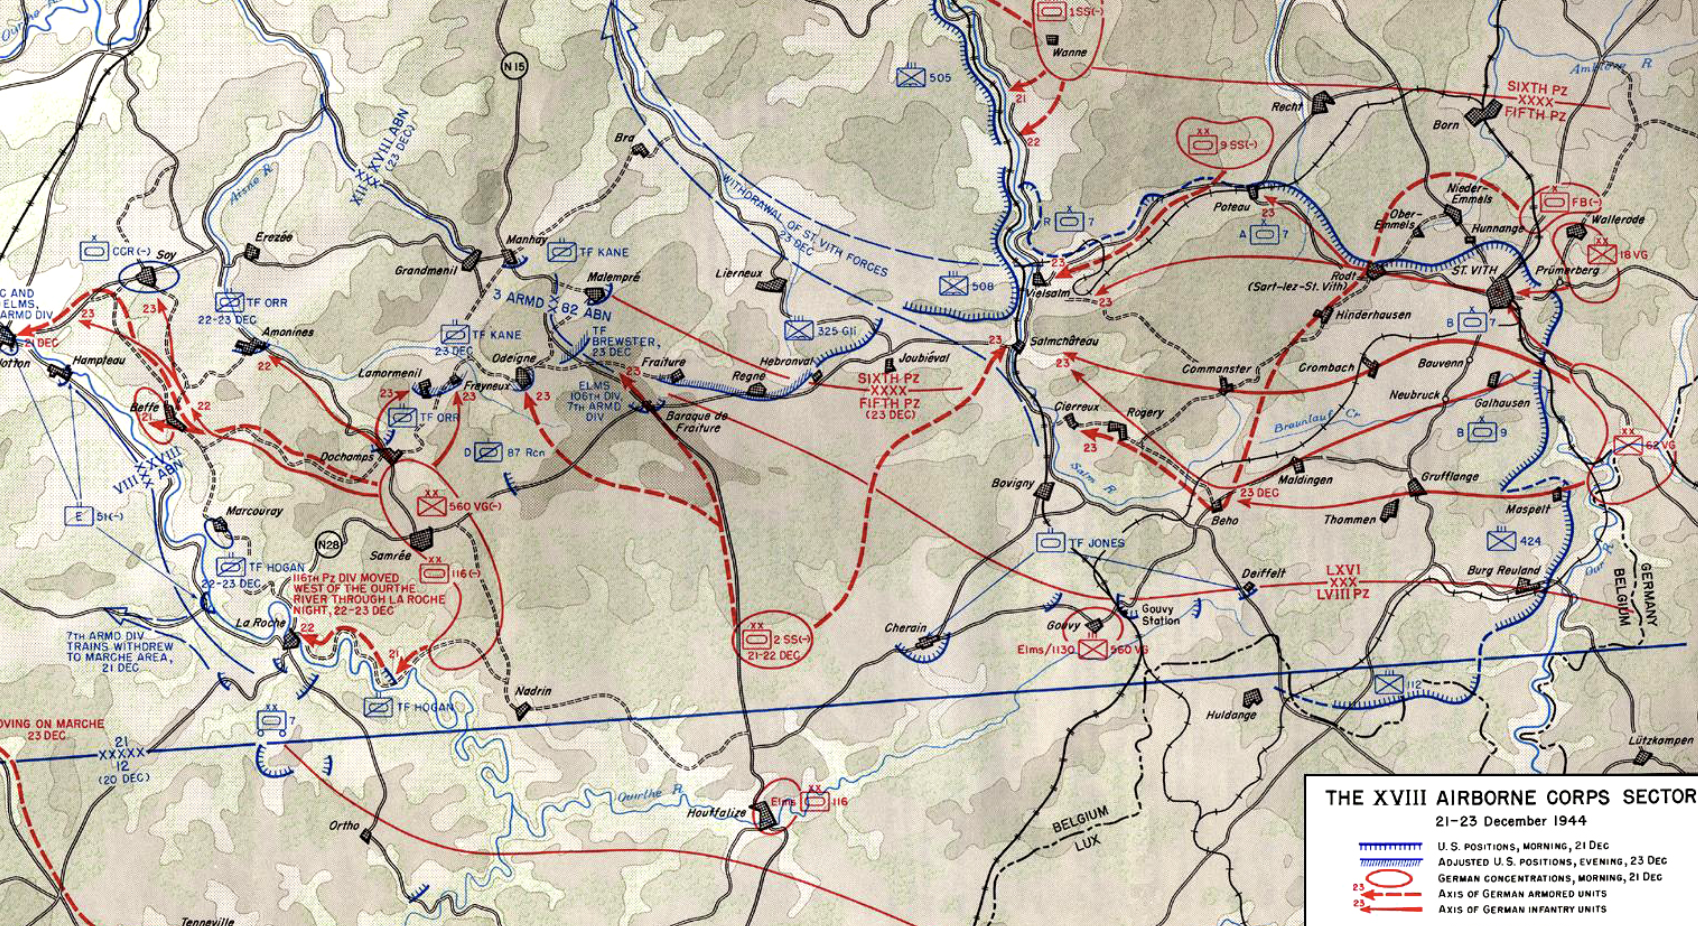
\includegraphics[width=.9\linewidth]{./example.org_imgs/g14eJd20240804T153654.png}
\caption{Ardennes, Battle of the Bulge, from \url{https://history.army.mil/books/wwii/7-8/notes/MapVII.jpg}.}
\end{figure}
\section{Enclosures}
\label{sec:org1762e9d}
\begin{itemize}
\item more stuff
\item additional extra stuff
\end{itemize}
\end{document}
